87. $\cfrac{(x+1)(x-2)^2}{x+2}\leqslant x^2-2x\Leftrightarrow \cfrac{(x+1)(x-2)^2-(x-2)x(x+2)}{x+2}\leqslant0\Leftrightarrow$\\
$\cfrac{(x-2)((x+1)(x-2)-x(x+2))}{x+2}\leqslant0\Leftrightarrow\cfrac{(x-2)(x^2-x-2-x^2-2x)}{x+2}\leqslant0
\Leftrightarrow \cfrac{(x-2)(3x+2)}{x+2}\geqslant0.$ Применив метод интервалов, найдём ответ: $x\in\left(-2;-\cfrac{2}{3}
ight]\cup[2;+\infty).$
\begin{figure}[ht!]
\center{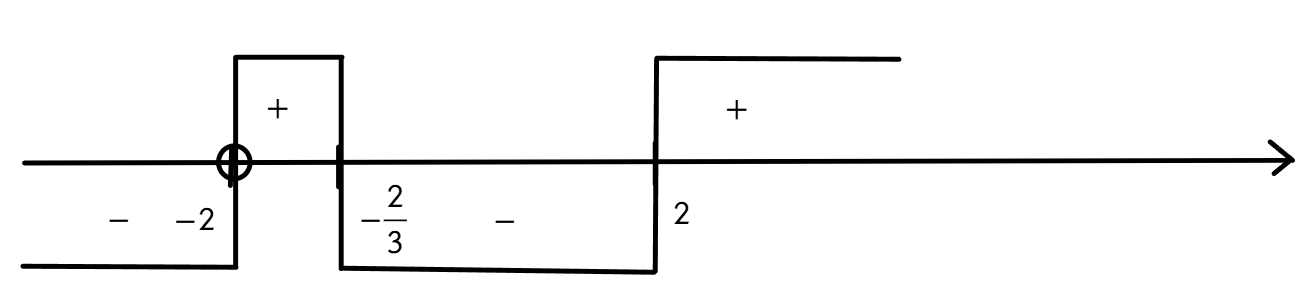
\includegraphics[scale=0.35]{ner9-85.png}}
\end{figure}\\
